\documentclass[11pt]{article}
\usepackage[margin=0.8in]{geometry}
\usepackage{amsmath,booktabs,graphicx,xcolor,hyperref}
\hypersetup{colorlinks=true,urlcolor=blue}
\definecolor{navy}{HTML}{17324D}
\setlength{\parindent}{0pt}
\setlength{\parskip}{6pt}
\begin{document}
{\LARGE\bfseries\color{navy} Coding Assignment 1}\par
{\large ECE 414/517 --- Dynamic Programming on RiverSwim}\par
\vspace{2pt}\hrule\vspace{6pt}
\textbf{Setup.} The supplied six-state model starts at $s_0$ (array index 0).
Action 0 is LEFT and action 1 is RIGHT. LEFT at $s_0$ pays $0.005$;
RIGHT at $s_5$ pays $1$. Values are expected infinite-horizon discounted
returns. Value iteration and the policy-evaluation step use synchronous
updates, stopping when the maximum absolute change in the value vector is
at most $10^{-10}$. Policy iteration stops when its policy is unchanged.
All supplied iteration limits are retained. Greedy ties select the smallest action index.

\textbf{(a) Largest grid discount selecting LEFT.}
I evaluated every discount in
$\{0.00,0.01,\ldots,0.99\}$ for every current strength.
The initial action is LEFT through the second column of the table and
RIGHT from the third column onward on this grid.
These are \emph{grid thresholds}, not exact continuous switching points.
The corresponding switching intervals are $[0.61,0.62]$, $[0.71,0.72]$,
and $[0.92,0.93]$ for weak, medium, and strong currents.
\begin{center}
\begin{tabular}{lrrrr}
\toprule
Current & Last LEFT $\gamma$ & First RIGHT $\gamma$ & $V^*(s_0)$ at .99 & $V^*(s_0)$ at .999\\
\midrule
Weak & 0.61 & 0.62 & 73.471119 & 843.931942 \\
Medium & 0.71 & 0.72 & 47.388319 & 587.773891 \\
Strong & 0.92 & 0.93 & 3.223457 & 46.106373 \\
\bottomrule
\end{tabular}
\end{center}
The $.999$ values come from the graduate-extension grid. At both $.99$
and $.999$, the optimal policy for all three currents is
$[1,1,1,1,1,1]$: choose RIGHT in every state.

\textbf{(b) Policy iteration versus value iteration.}
Both methods converge for every tested setting and return identical
six-state policy arrays in all 300 required-grid cases and all 150
extension cases. The maximum absolute difference between their value
vectors, over all states and discounts, is shown below.
\begin{center}
\begin{tabular}{lrr}
\toprule
Current & Required grid & Extension grid\\
\midrule
Weak & $7.82\times 10^{-14}$ & $1.07\times 10^{-14}$ \\
Medium & $1.44\times 10^{-12}$ & $2.50\times 10^{-13}$ \\
Strong & $8.12\times 10^{-11}$ & $9.31\times 10^{-11}$ \\
\bottomrule
\end{tabular}
\end{center}
The overall difference is $9.31\times 10^{-11}$.
As an independent numerical check, each returned policy was evaluated with
$(I-\gamma P^\pi)^{-1}r^\pi$ using a linear-system solve and confirmed greedy
with respect to those values. Across both methods and both grids, the
largest optimal Bellman residual is $9.99\times 10^{-11}$ and the largest difference
from direct evaluation is $9.99\times 10^{-8}$.
The stopping tolerance bounds successive updates, not the exact value
error: the contraction bound is approximately
$10^{-10}/(1-\gamma)$, or $10^{-7}$ at $\gamma=.999$.

\textbf{(c) Effect of stronger current.}
The RIGHT dynamics list backward, stay, and forward probabilities:
weak $(.05,.60,.35)$, medium $(.10,.65,.25)$, and strong $(.15,.75,.10)$.
The interior expected displacement under RIGHT
therefore decreases from $+.30$ to $+.15$ to $-.05$ states per step.
Reaching and remaining near the larger right-boundary reward becomes harder,
so a longer effective horizon is needed to justify leaving the small
guaranteed reward on the left. The largest LEFT discount increases by
$0.10$ from weak to medium and by another $0.21$ from medium to strong.
At a fixed sampled discount, $V^*(s_0)$ never increases with current strength:
it is weak $\geq$ medium $\geq$ strong on both grids. At $.99$ the strong-current
value is 95.6\% below the weak-current value.

\newpage
{\Large\bfseries\color{navy} Graduate extension and reproducibility}\par
\textbf{ECE 517 extension.}
I evaluated 50 evenly spaced discounts using
\texttt{np.linspace(0.80, 0.999, 50)} for each current strength.
This includes both endpoints and exceeds the required 20 points.
The figure plots the initial optimal value from value iteration;
policy iteration gives the same curves to numerical precision.

\begin{center}
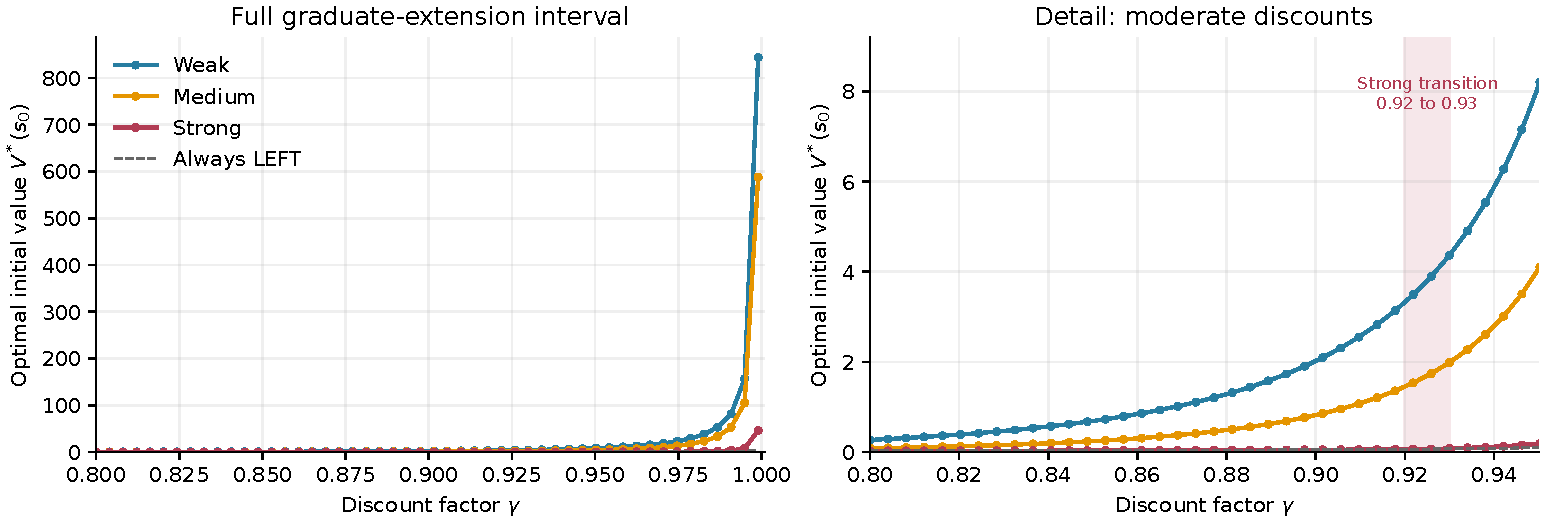
\includegraphics[width=\linewidth]{values_vs_discount.pdf}
\end{center}
{\small Each colored marker is one of the 50 tested discounts. The right
panel enlarges the moderate-discount range; the shaded band brackets the
strong-current transition on the required $0.01$ grid. The dashed curve
is the value of staying at $s_0$ and choosing LEFT forever.}\par

For weak and medium currents, all 50 extension discounts choose RIGHT
at $s_0$. For the strong current, 31 choose LEFT and
19 choose RIGHT. Whenever LEFT is optimal at the initial state,
the agent remains there and receives $V^*(s_0)=0.005/(1-\gamma)$.
For example, all three currents have value $0.0125$ at $\gamma=.60$;
the stronger currents separate only when swimming right becomes worthwhile.

As $\gamma$ approaches 1, future rewards retain more weight and the
effective horizon $1/(1-\gamma)$ grows from 5 at $.80$ to 1,000 at $.999$.
Repeated rewards at the right boundary then compensate for travel delays,
even against the strong current. All three values rise sharply, while the
weak current still yields the highest return because it reaches and occupies
the right boundary more easily. The strong-current value remains
94.5\% below the weak-current value at $.999$.
The LEFT baseline also diverges as $\gamma$ approaches 1, so rising value
alone does not imply a policy change; the relative action values determine it.
\end{document}
